\documentclass[10pt,a4paper,notitlepage]{article}
\usepackage[utf8]{inputenc}
%\usepackage[francais]{babel}
\usepackage[T1]{fontenc}
\usepackage{amsmath}
\usepackage{amsfonts}
\usepackage{amssymb}
\usepackage{graphicx}
\usepackage{hyperref}
\usepackage[left=2cm,right=2cm,top=2cm,bottom=2cm]{geometry}
\author{Mercier Wilfried}

\graphicspath{{../../Plots/}}

\begin{document}

\section{Comparaison des magnitudes}

    \begin{figure}[h]
	    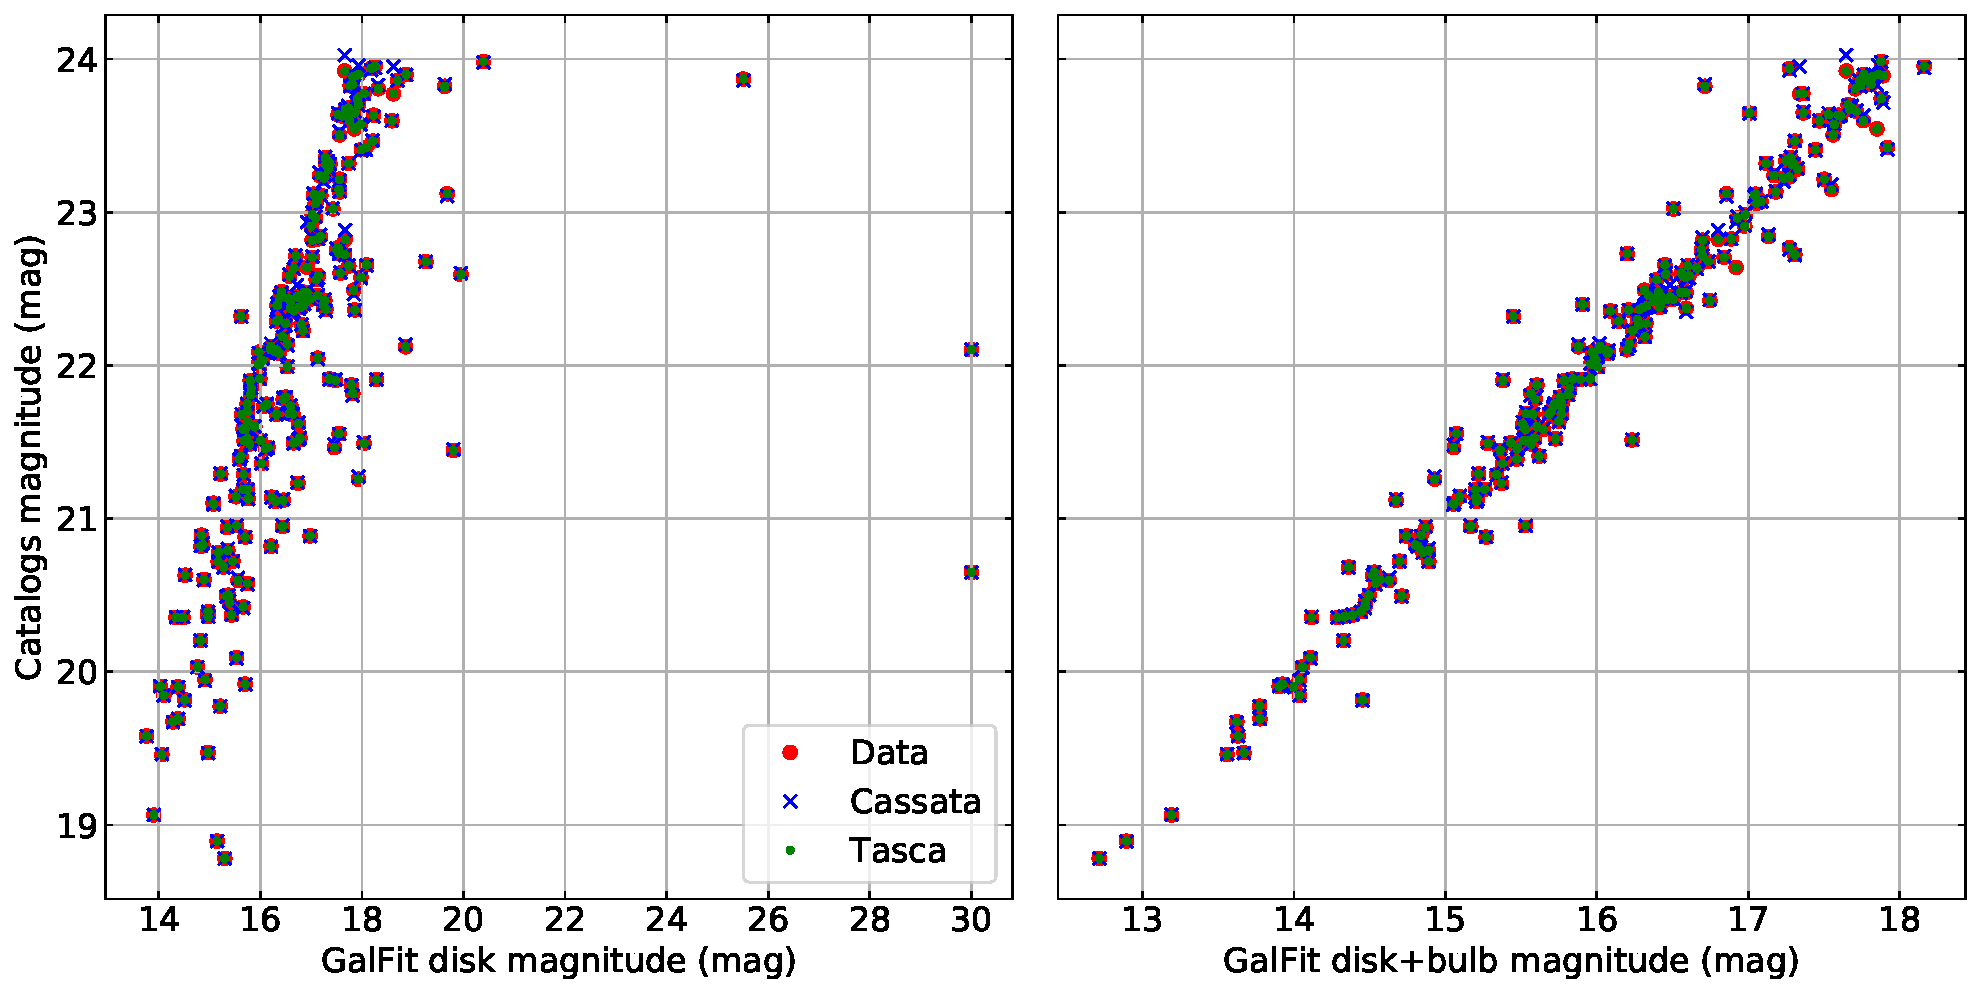
\includegraphics[width=\linewidth]{catalogMag_against_GalfitMag_corrected.pdf}	
	    \caption{Gauche : comparaison des magnitudes fournies dans les catalogues avec celle du disque retournée par GalFit. Droite : même graphe avec la magnitude totale disque+bulbe comme décrite en Eq\,\ref{eq:mag_tot}.}
    \end{figure}
    
    Les magnitudes entre les catalogues sont les mêmes et sont cohérentes avec celle de GalFit si on prend la combinaison du bulbe et du disque, i.e.
    
    \begin{equation}
        \label{eq:mag_tot}
        m^{\rm{GF}}_{\rm{d+b}} = -2.5 \log_{10}\left [ 10^{-\frac{m_d}{2.5}} + 10^{-\frac{-m_b}{2.5}} \right ]
    \end{equation}
    où $m_d$ et $m_b$ sont respectivement les magnitudes du disque et du bulbe retournées par GalFit.    
    
    On retrouve bien un relation linéaire de pente 1 avec un offset probablement dû à une calibration ou une constante du système de magnitude utilisée différente.
    
    \newpage
    
    \section{Comparaisons des types de galaxies entre catalogues}
    
    Chaque catalogue fournit un type aux galaxies (elliptique, disque, irrégulière). Cassata et Zurich en donne un seul et Tasca en donnent trois (Int avec une méthode similaire à Cassata, Linee en utilisant la méthode ACS, SVM avec du machine learning).
    
    Les meilleurs correspondances sont pour Tasca Int/Tasca Linee avec Cassata (cf. Fig\,\ref{fig:types}). Zurich trouve qu'un grand nombre de galaxies elliptiques de Cassata sont en réalité des disques. 
    
    Les types de Cassata ont donc été utilisé dans la suite.
    
    \begin{figure}[h]
        \centering
	    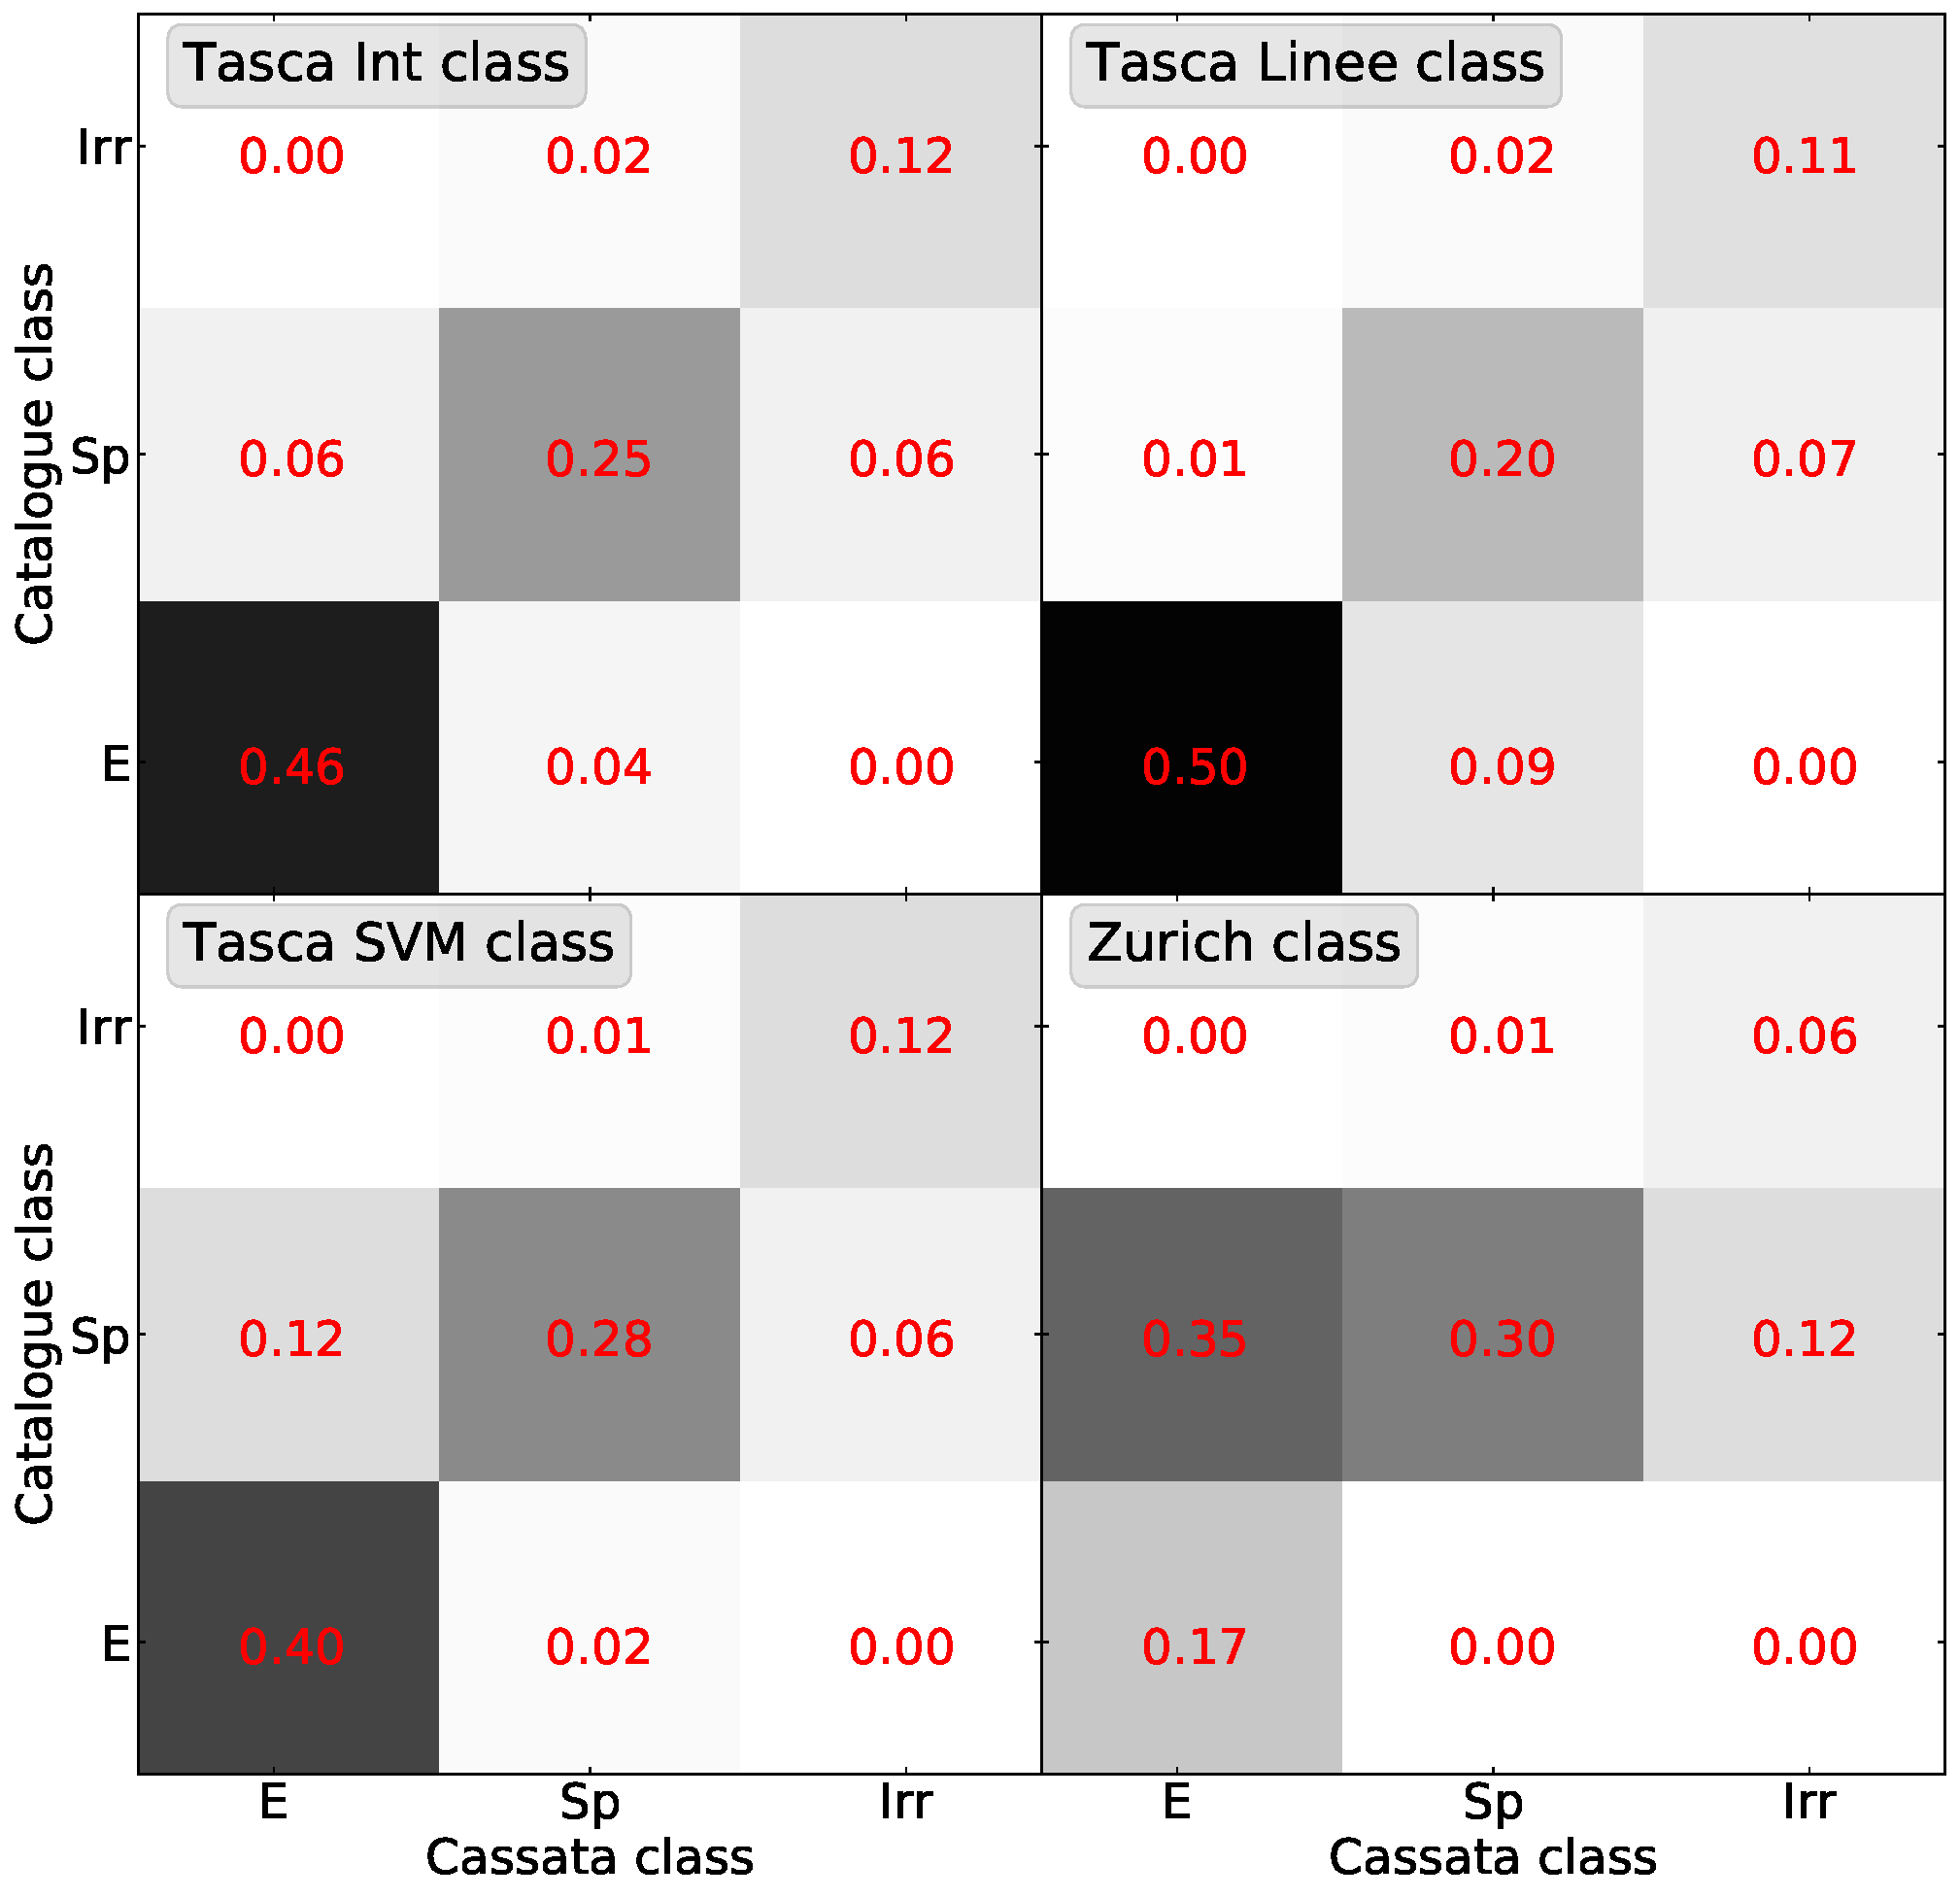
\includegraphics[width=0.8\linewidth]{comparisonClassTypes.pdf}	
	    \caption{Histogramme des types des galaxies trouvés par les catalogues (E pour elliptique, Sp pour disque/spirale, Irr pour irrégulière). Plus la couleur est foncée, plus il y a d’occurrences. Le nombre exact dans chaque case est représenté par dessus.}
	     \label{fig:types}
    \end{figure}
    
    
    \newpage
    
    \section{Différence entre rayons des catalogues et celui de GalFit}
        \subsection{Comparaison en utilisant le rayon du disque de GalFit}
        
    \begin{figure}[h]
        \centering
         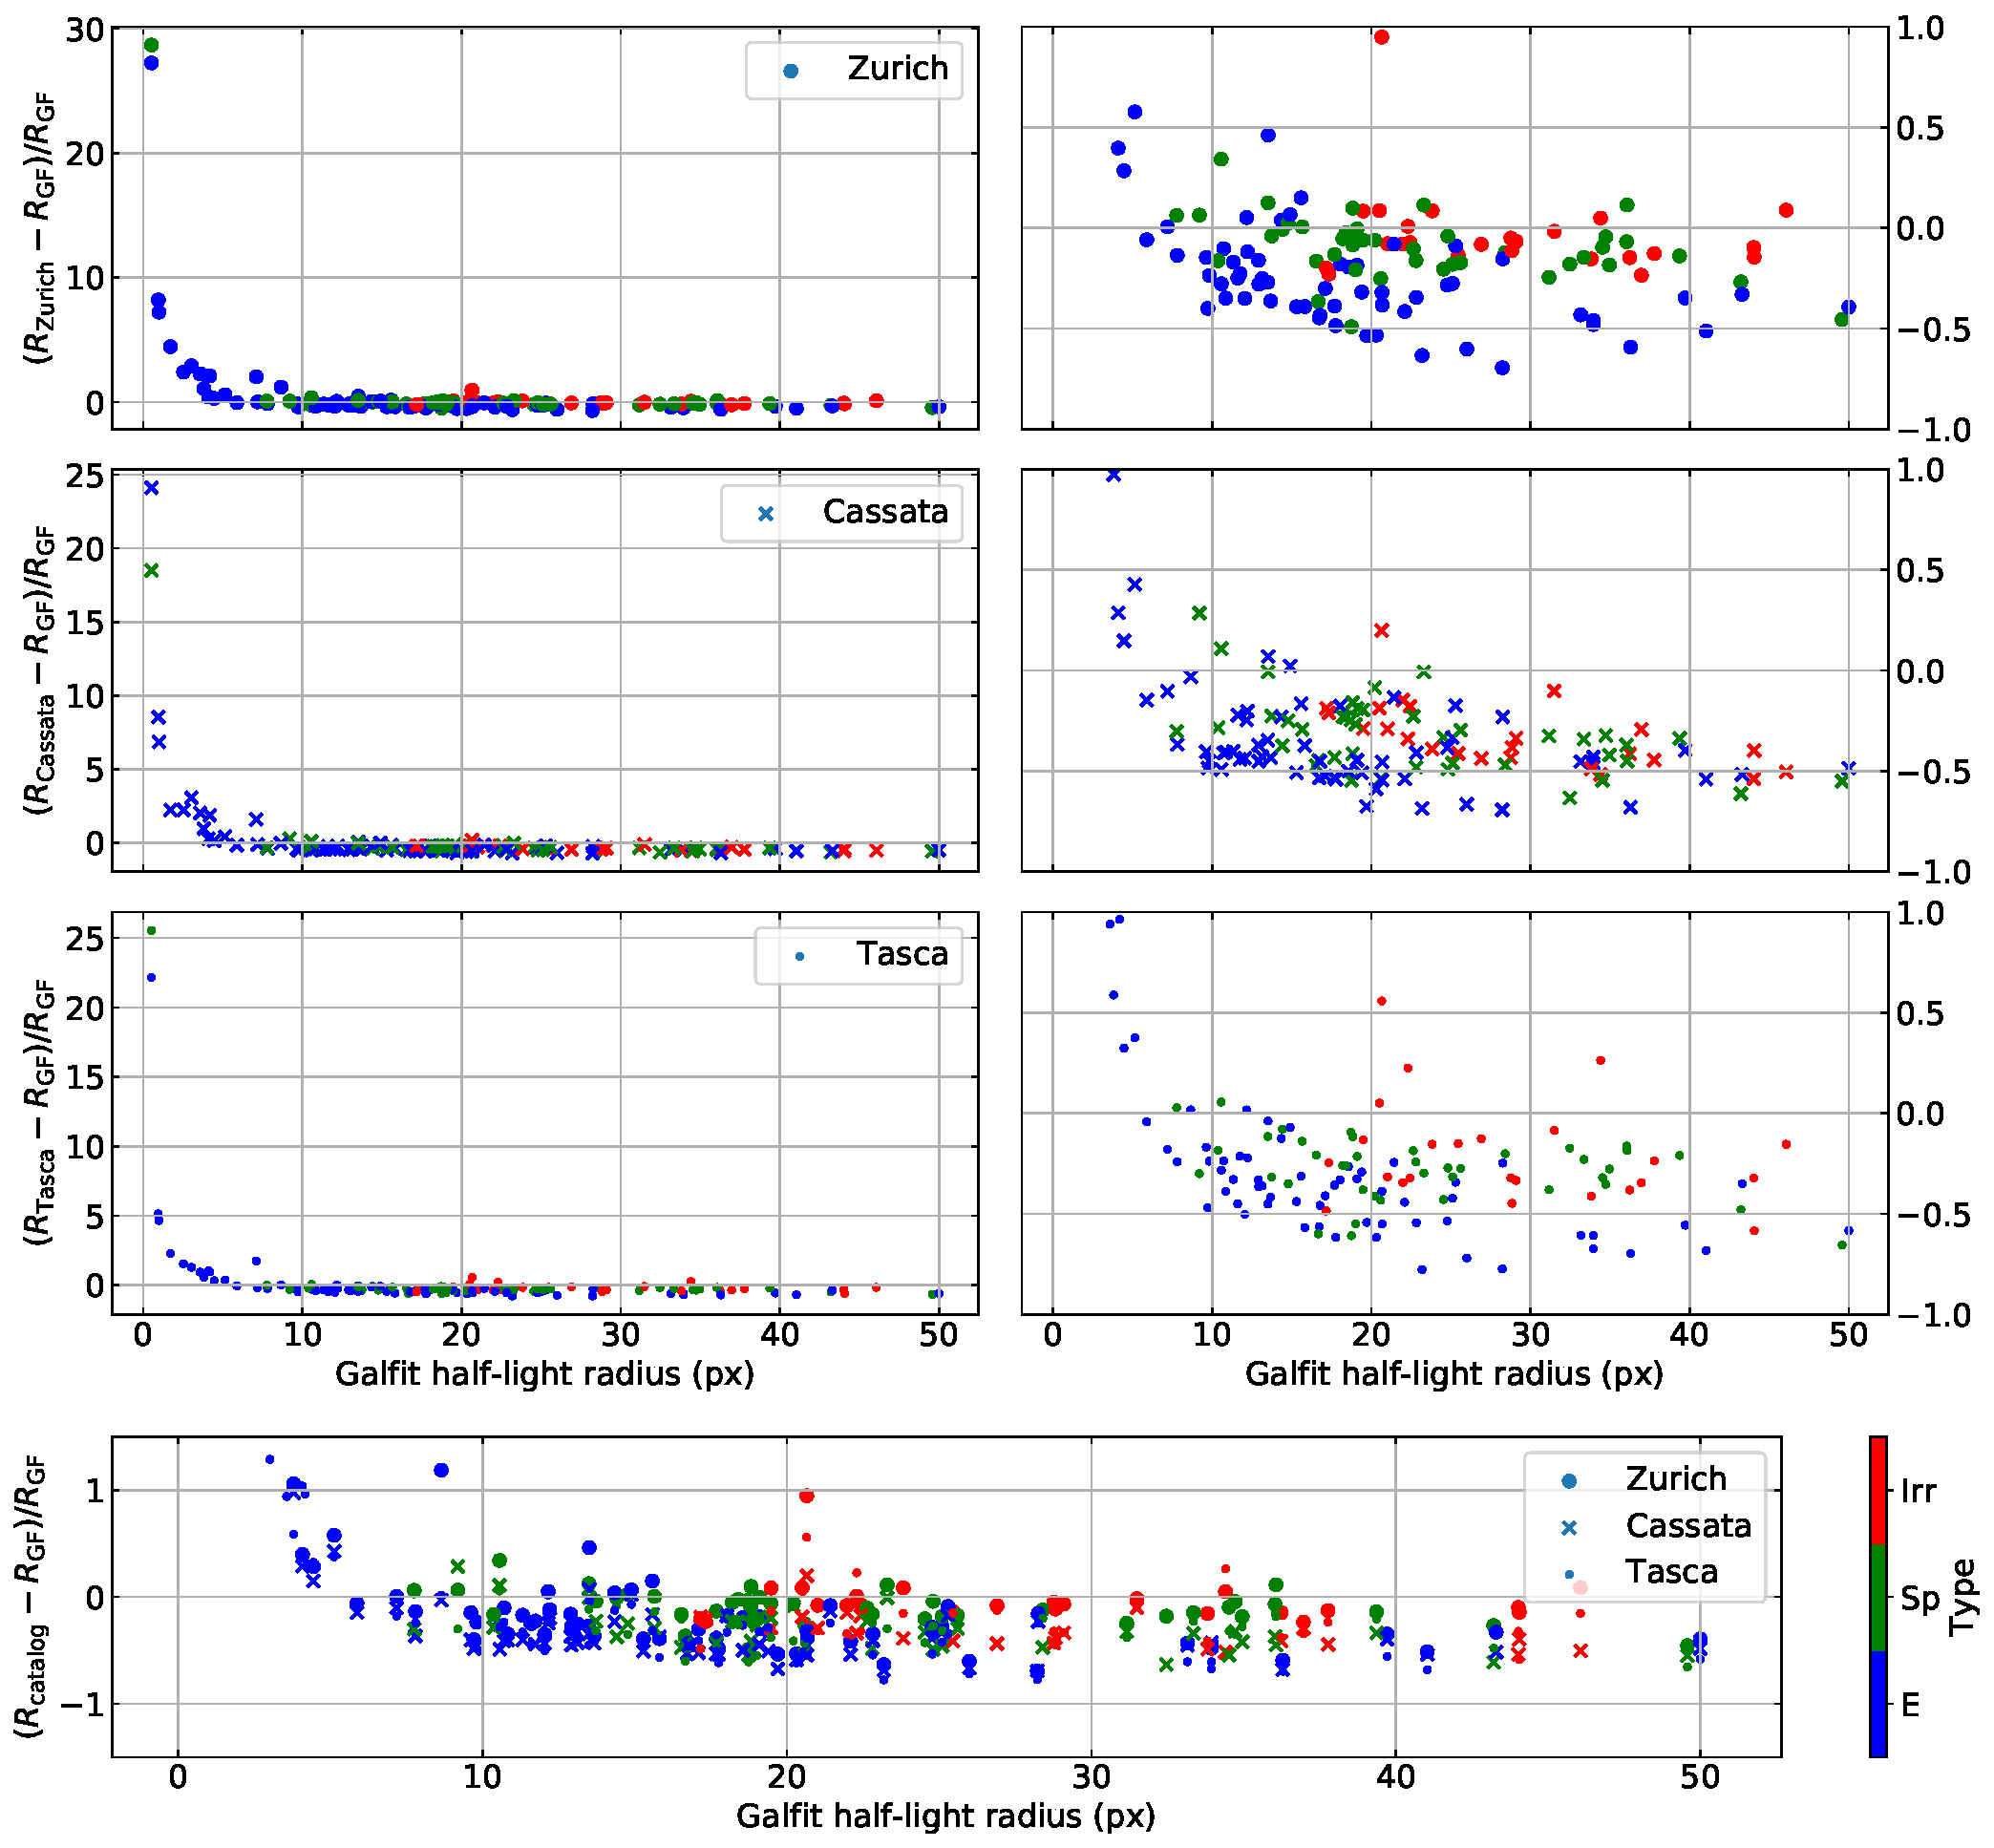
\includegraphics[width=0.8\linewidth]{{plotsWithColourCoding/relErr_against_GalFit1.5LightRadius_colourCoded_CassataType}.pdf}
	    \caption{Gauche : vue d'ensemble de la différence relative entre les rayons des catalogues et celui de GalFit (disque seulement). Droite : zoom sur les points autour de 0. Bas : Graphes avec les trois catalogues dans la même zone.}
	     \label{fig:delta_radii}
    \end{figure}     
    
    Le catalogue de Zurich semble donner la différence avec GalFit la moins prononcée pour les galaxies spirales/disques et irrégulières (respectivement symboles verts et rouges, cf. Fig.\,\ref{fig:delta_radii}). Le rayon GalFit des galaxies elliptiques est quant à lui surestimé d'environ 50\%. Prendre le rayon déconvolué au lieu du rayon effectif ne change pas la conclusion.
    
    Si on sépare les galaxies en trois groupes (E, Sp, Irr) avec les types trouvés par Zurich (cf. Fig.\,\ref{fig:delta_radii_zurichColour}), on trouve cette fois que les spirales sont biens plus dispersées autour de zéro avec un biais négatif (rayon effectif de GalFit surestimé par rapport à ceux des catalogues).
    
    On retrouve la même tendance lorsqu'on compare à la masse et à la magnitude(cf. Fig.\,\ref{fig:delta_mass} et \ref{fig:delta_mag}).

    \begin{figure}[h]
        \centering
         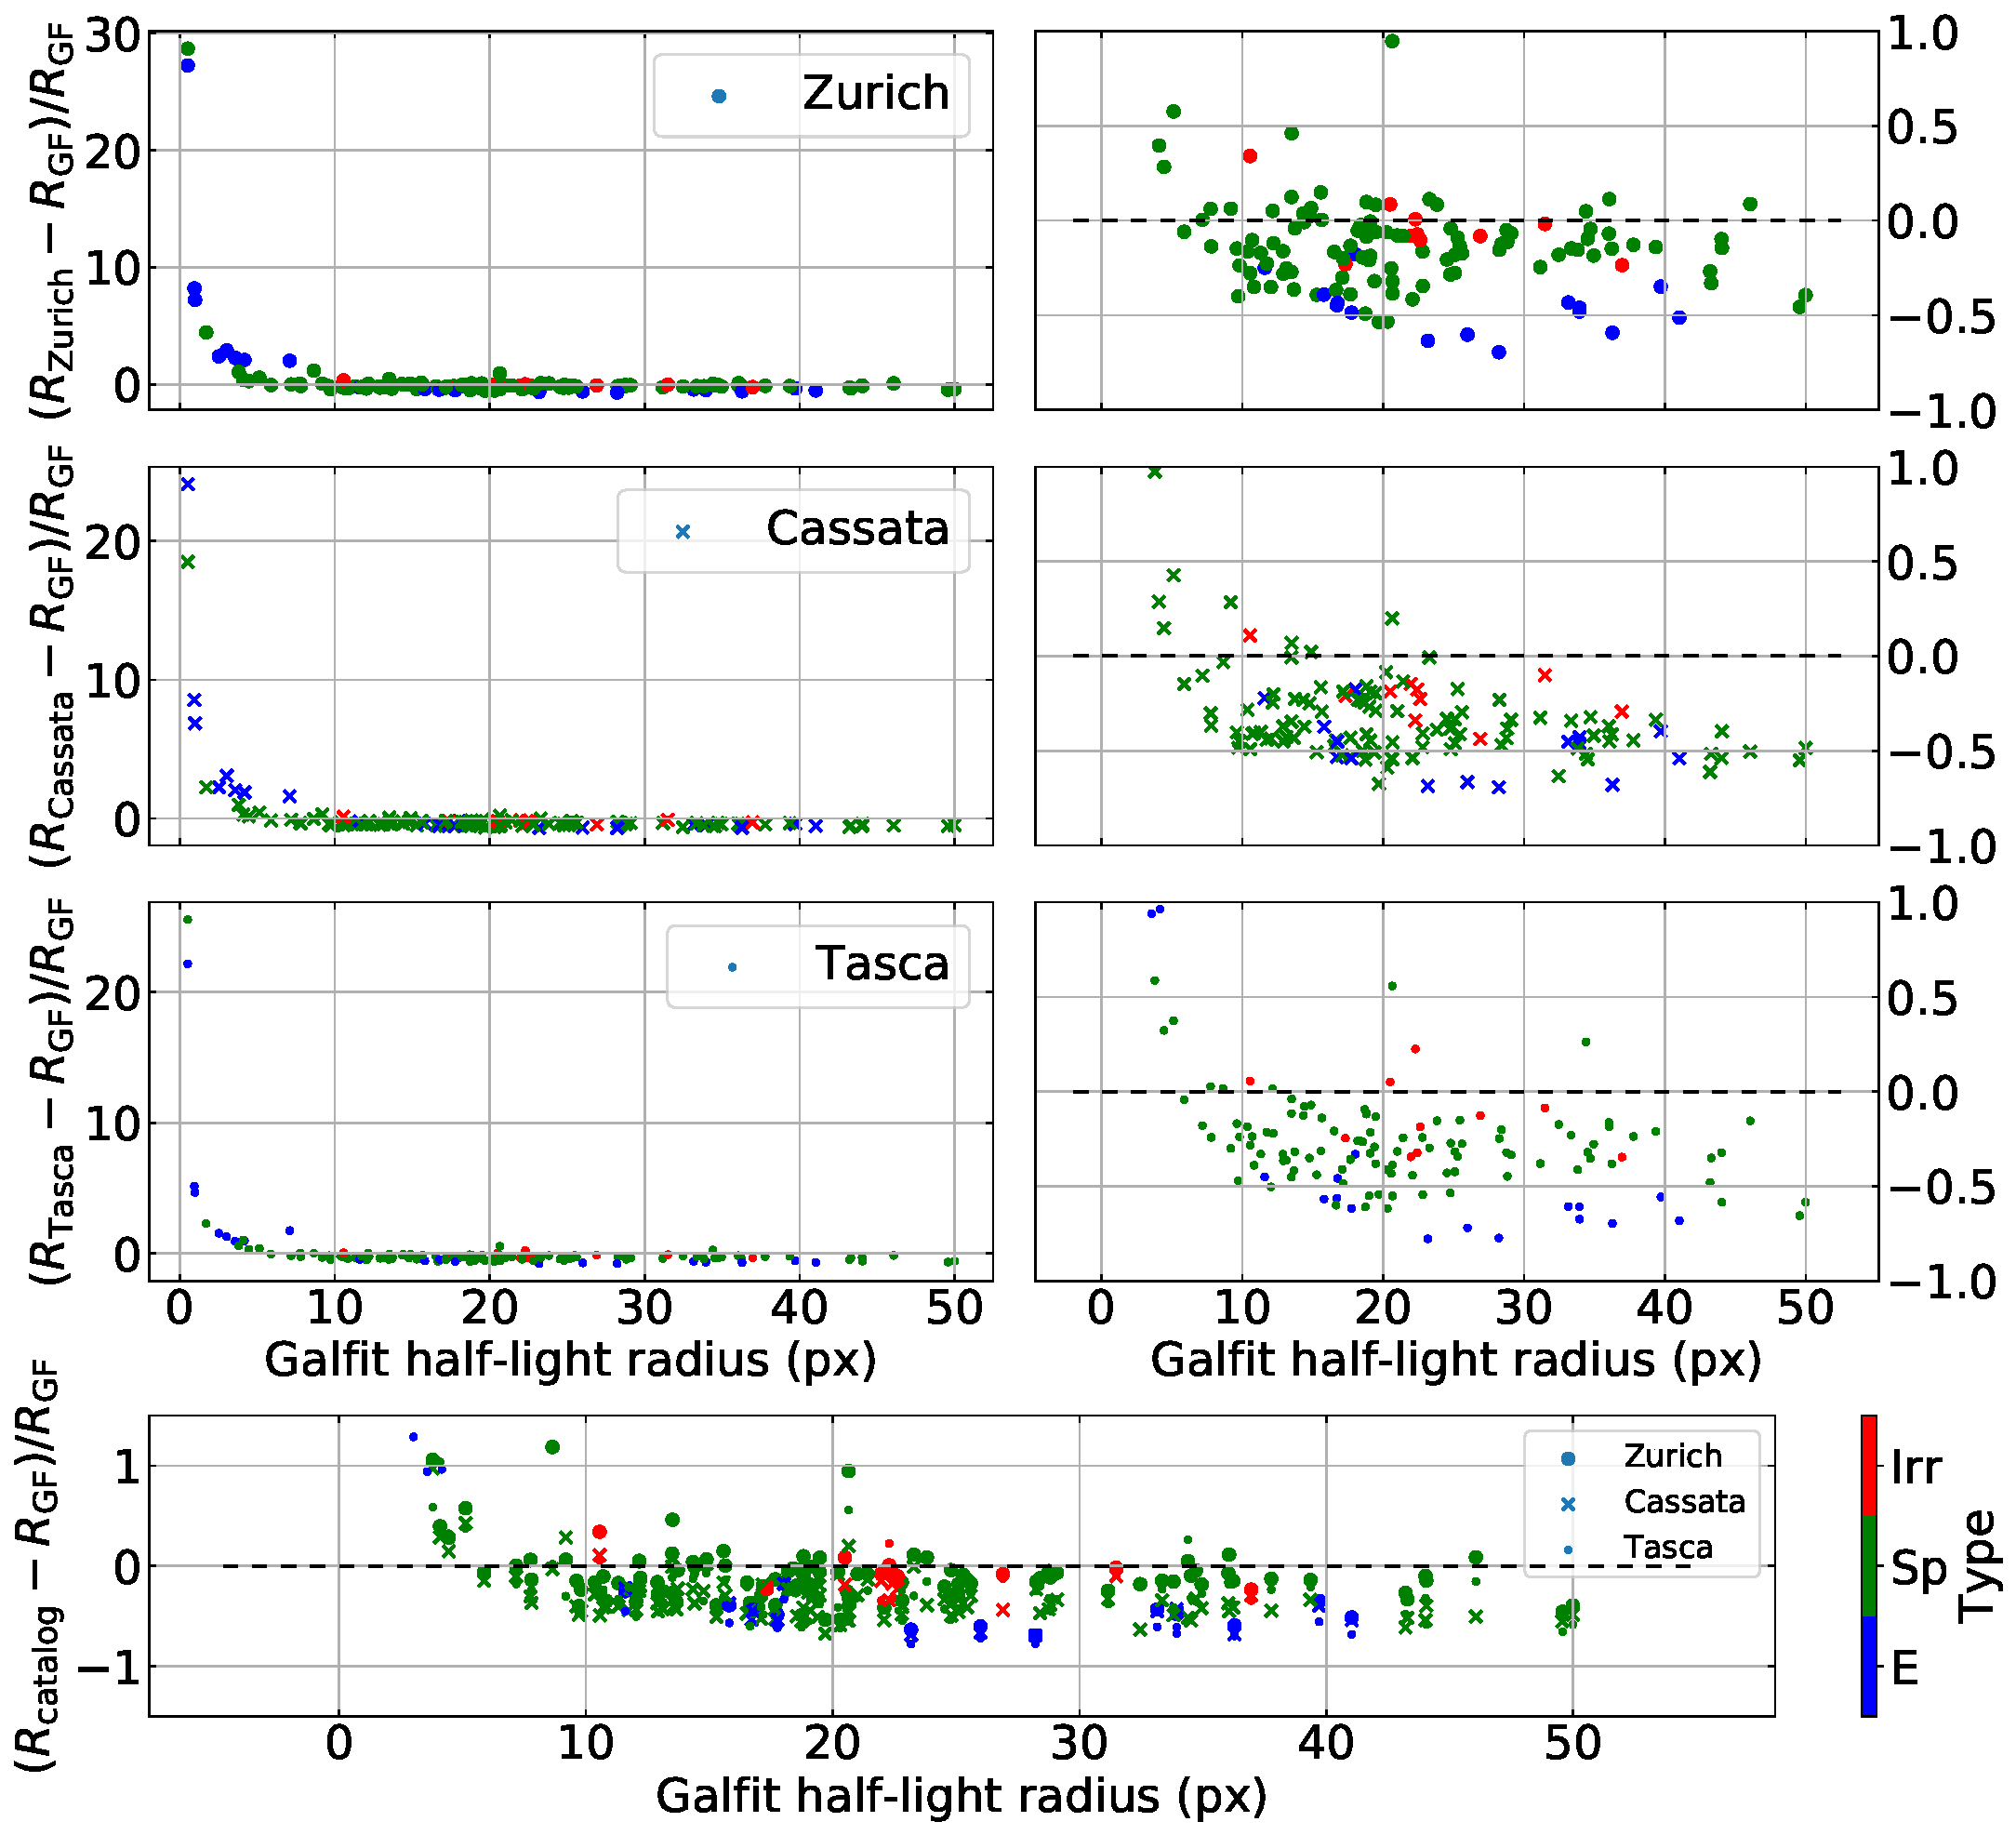
\includegraphics[width=0.7\linewidth]{{plotsWithColourCoding/relErr_against_GalFit1.5LightRadius_colourCoded_zurichType}.pdf}
	    \caption{Même graphe que Fig.\,\ref{fig:delta_radii} mais en utilisant les types de galaxies fournis par Zurich au lieu de Cassata.}
	     \label{fig:delta_radii_zurichColour}
	     
        \hfill	     
	     
	     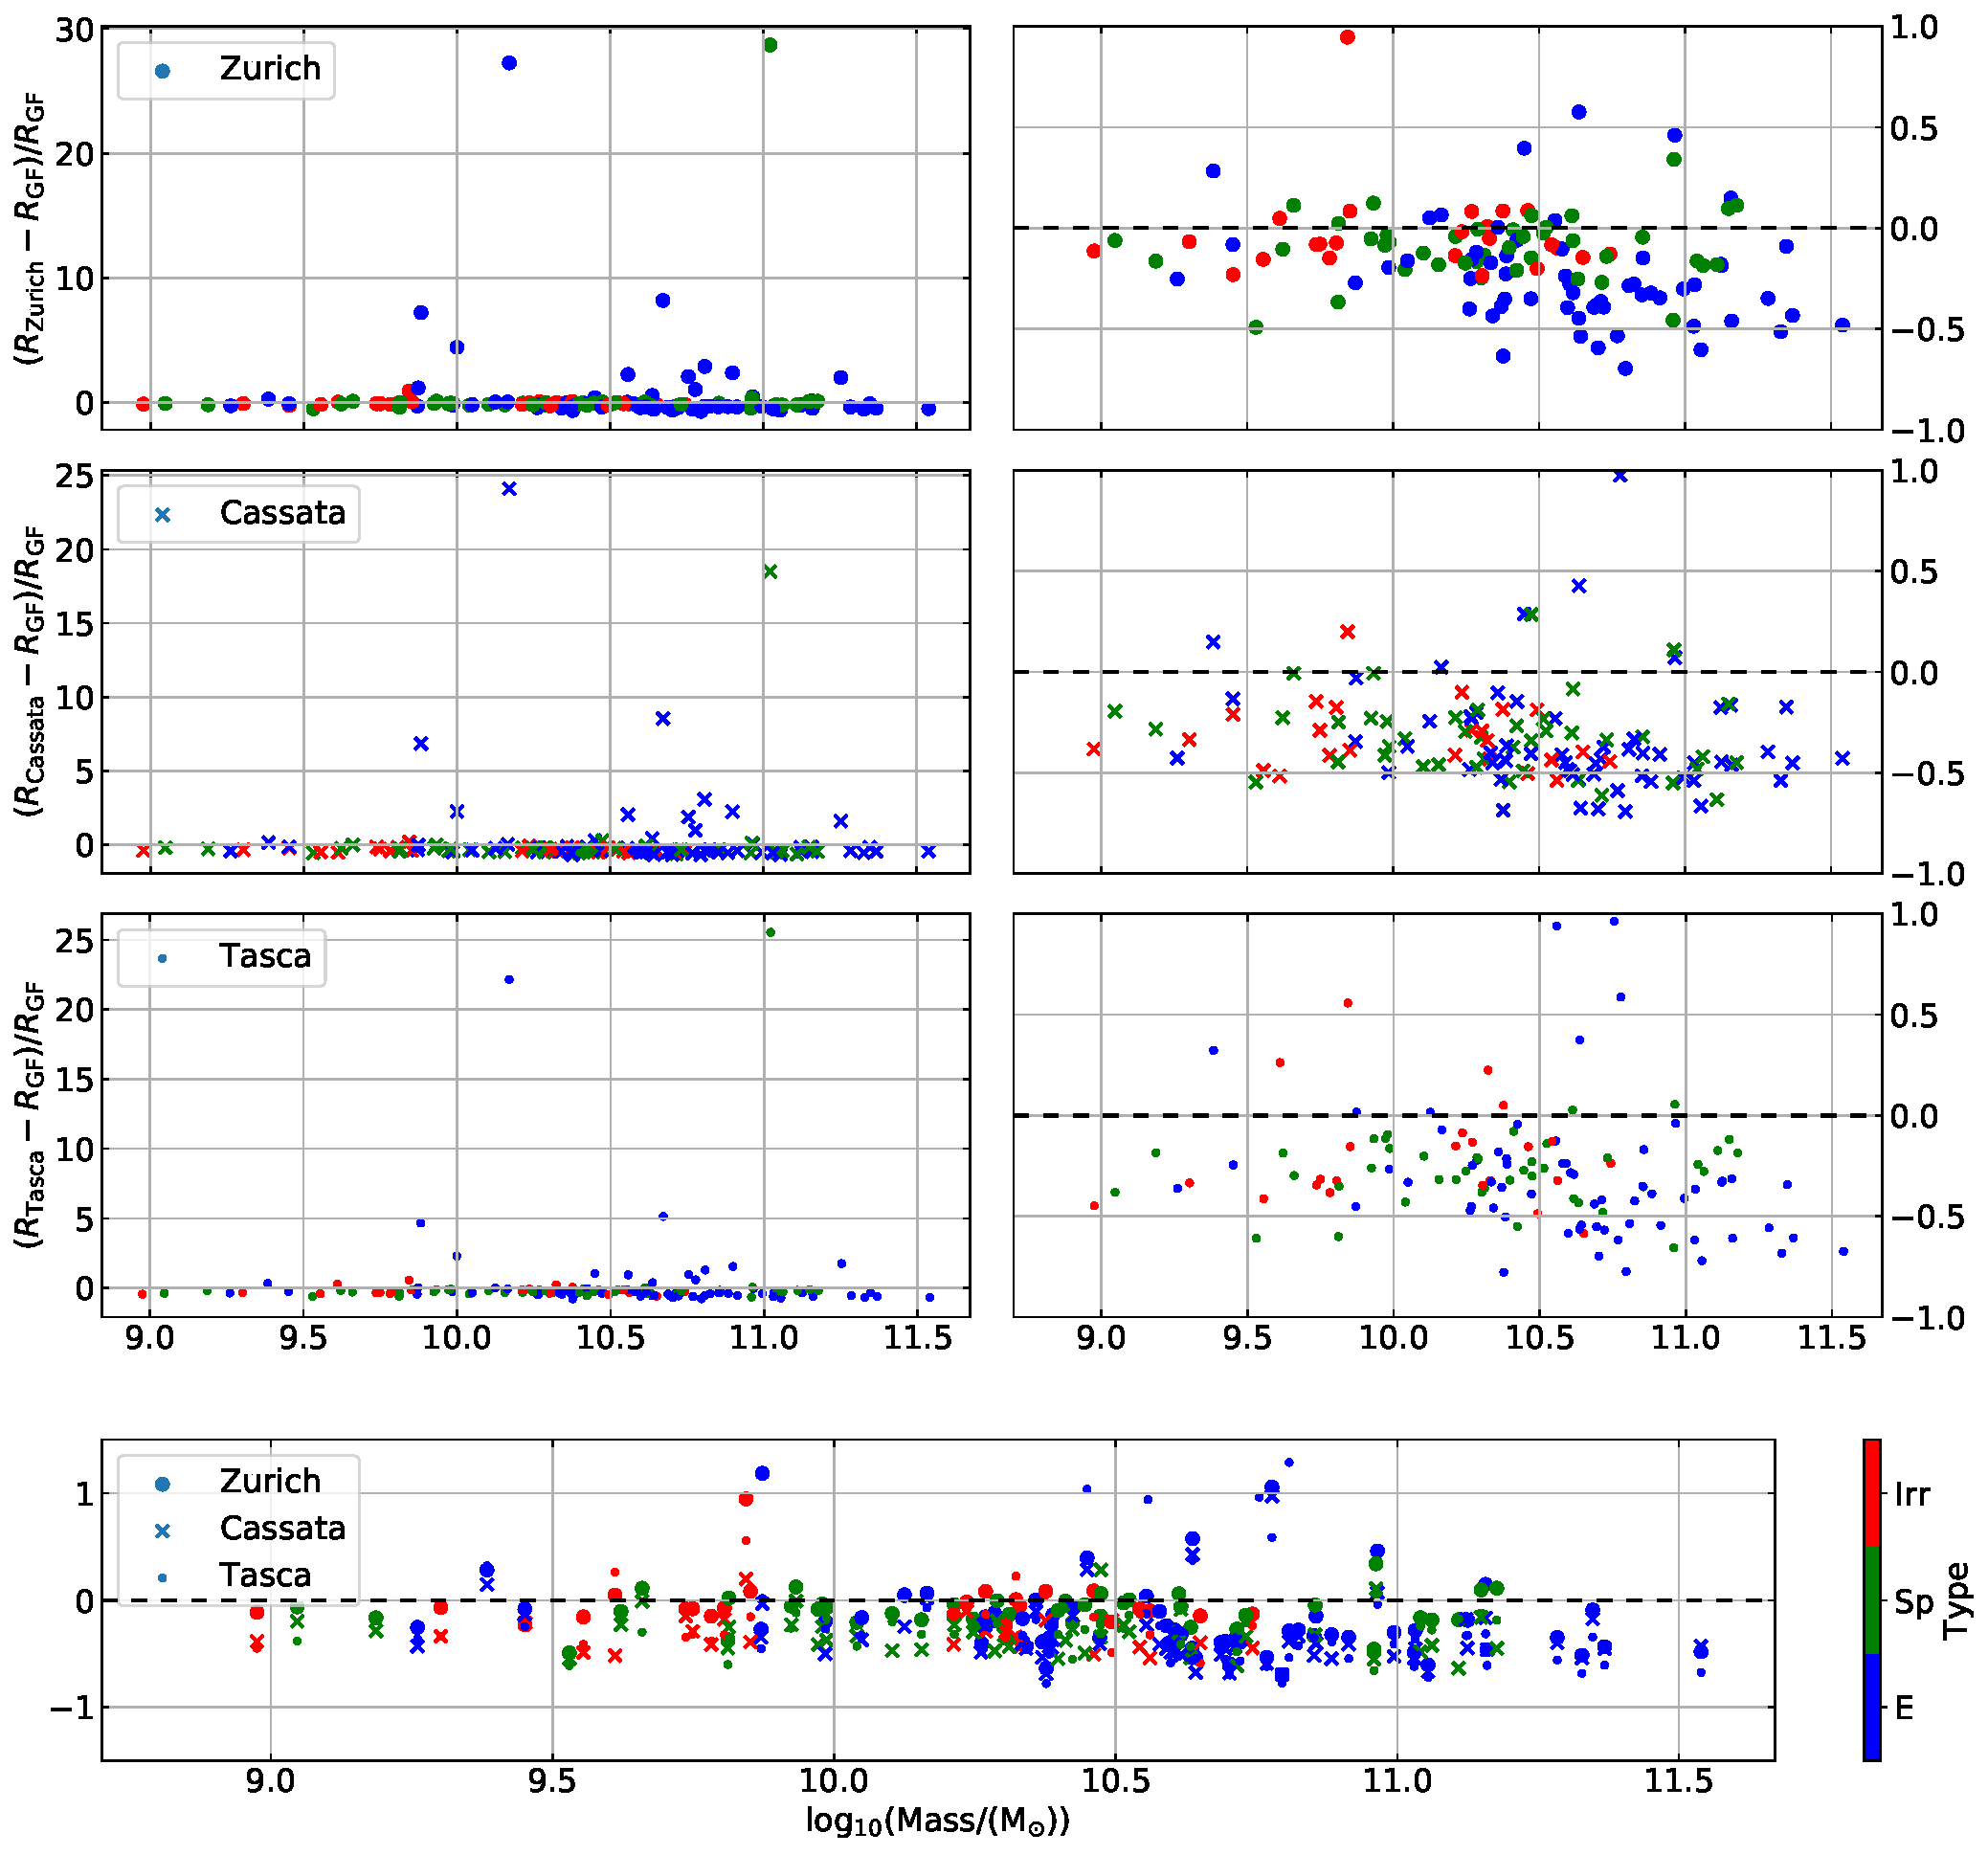
\includegraphics[width=0.7\linewidth]{{plotsWithColourCoding/relErr_against_mass_colourCodedWithCassataType}.pdf}
	    \caption{Différence relative du rayon en fonction de la masse des galaxies. Gauche : vue d'ensemble. Droite : zoom sur la partie située autour de 0. Bas : graphes avec les trois catalogues réunis. Le même code couleur que dans les graphes précédents est utilisé.}
	     \label{fig:delta_mass}
    \end{figure}     
    
    \begin{figure}[h]    
        \centering
	    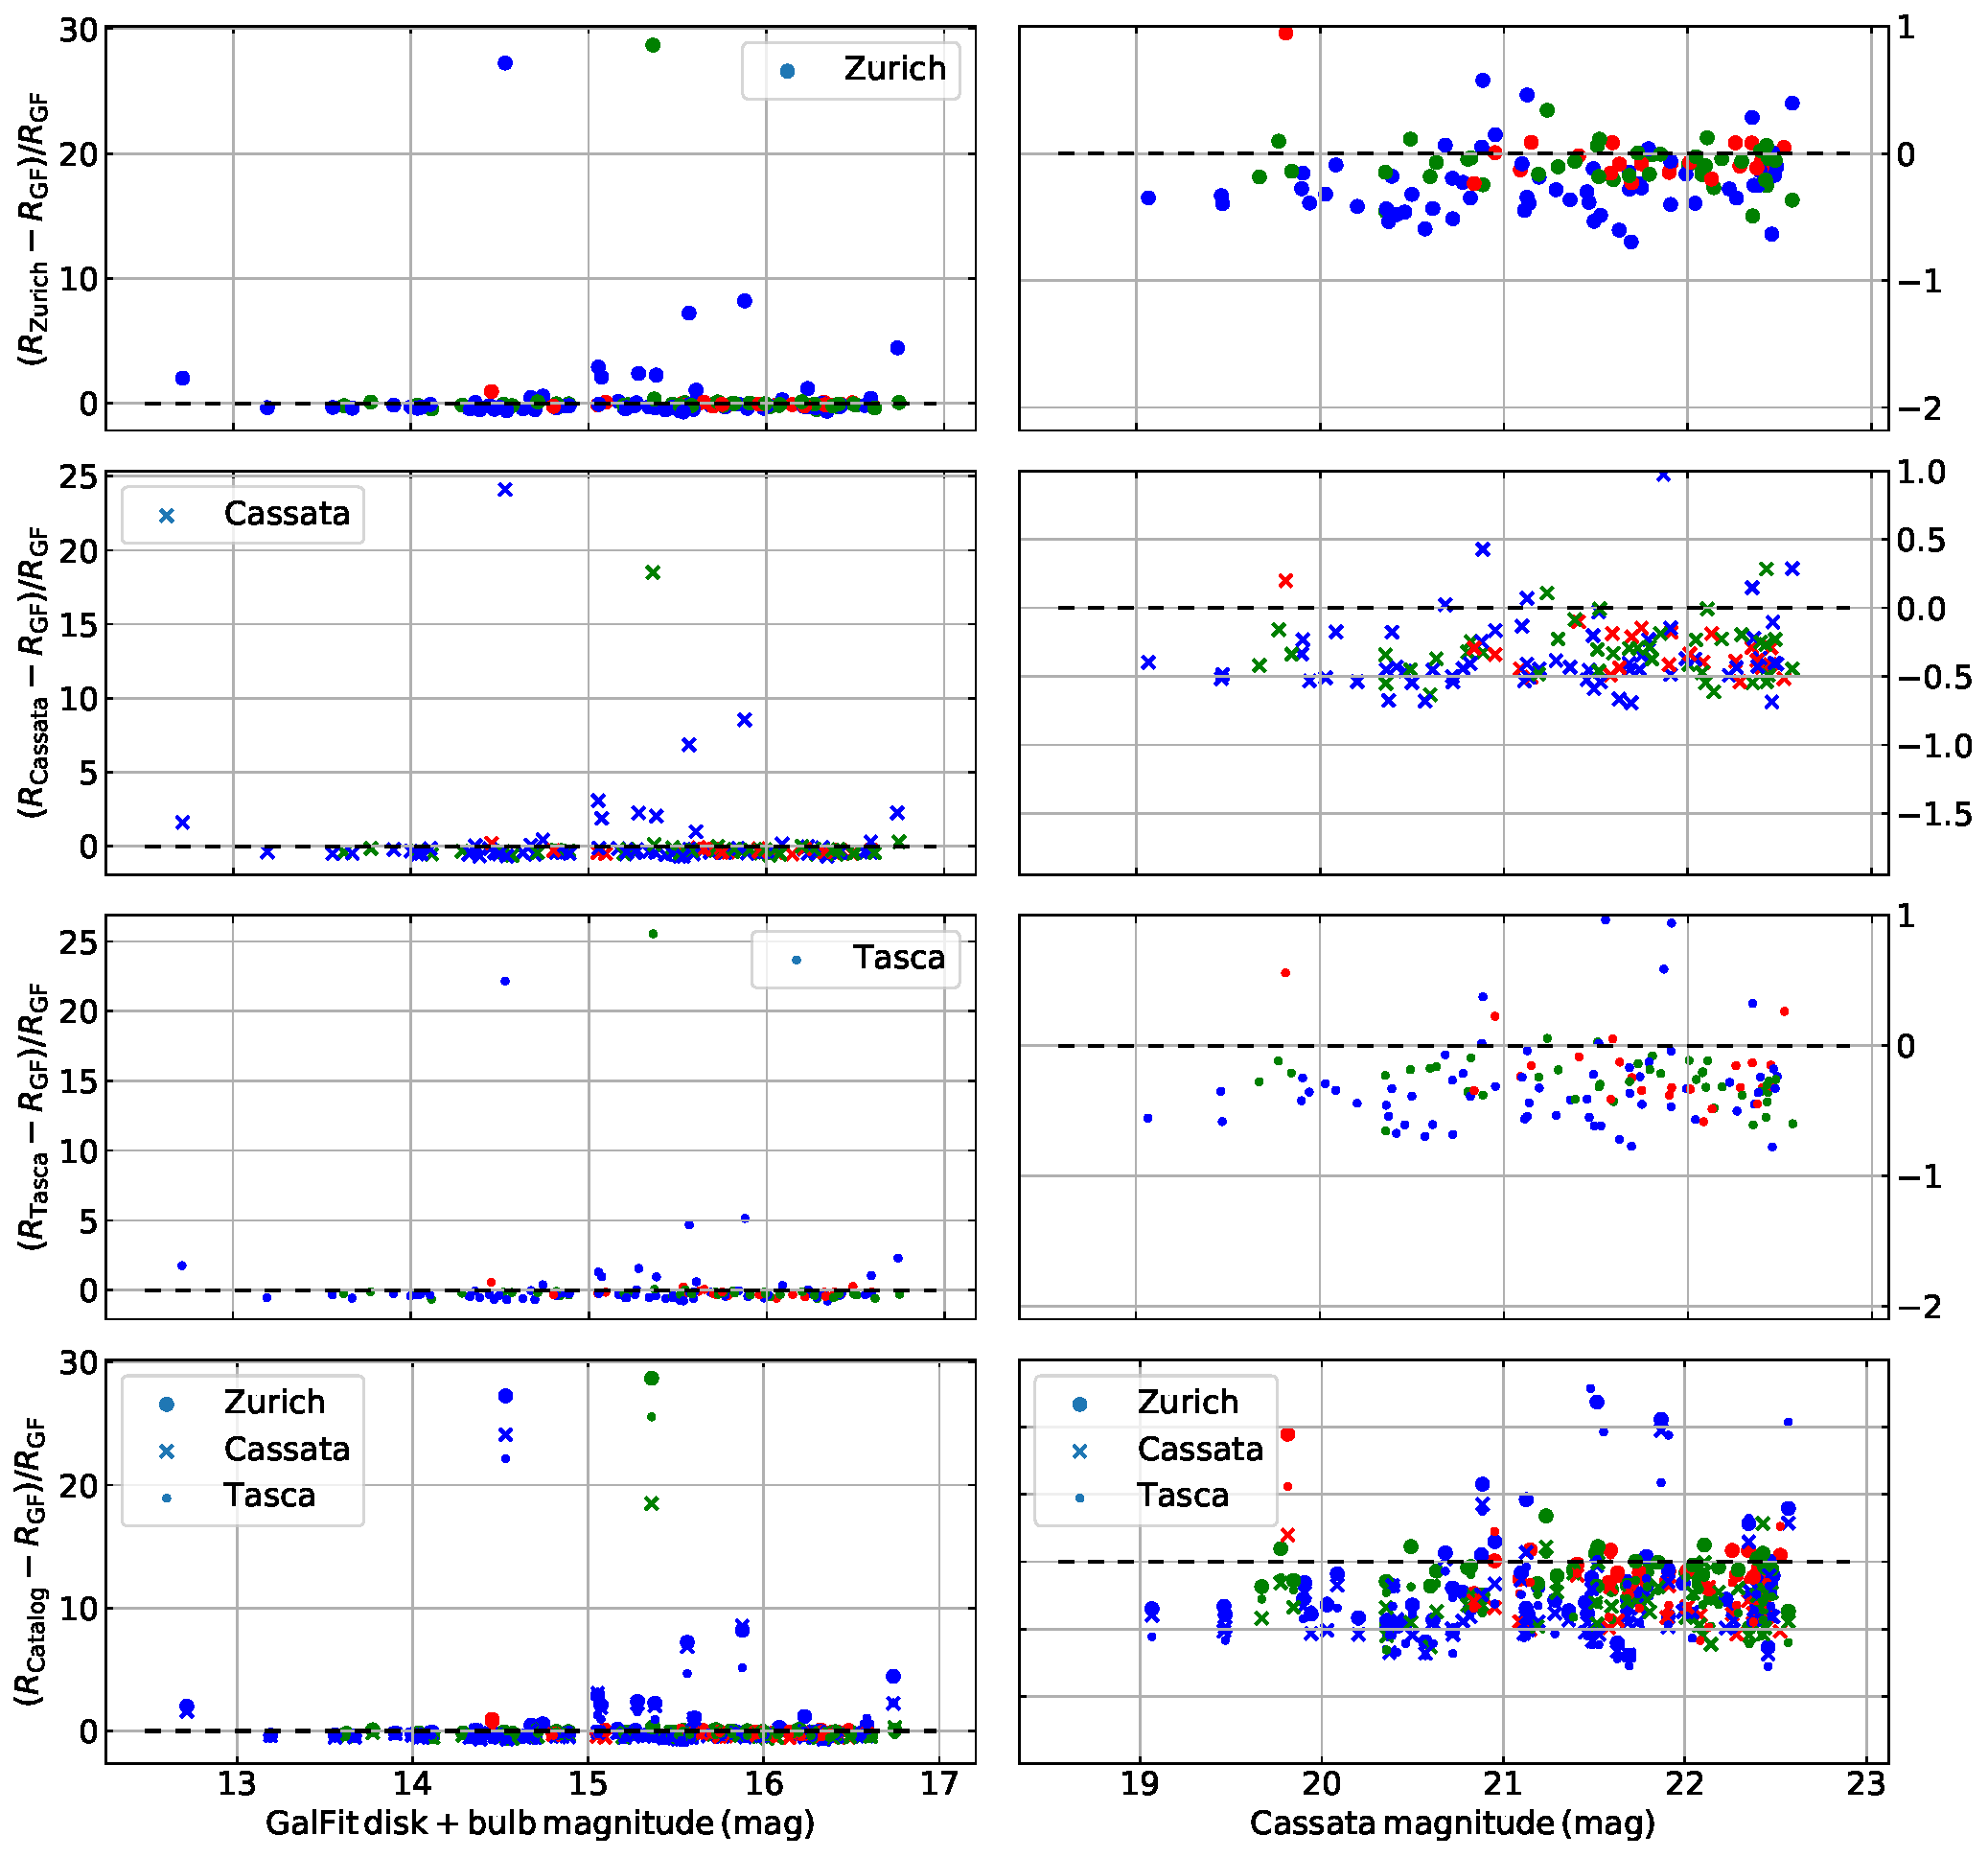
\includegraphics[width=0.8\linewidth]{{plotsWithColourCoding/relErr_against_mag_colourCodedWithCassataType}.pdf}
	    \caption{Différence relative du rayon en fonction de la magnitude totale (disque+bulbe) des galaxies fournie par GalFit. Gauche : vue d'ensemble. Droite : zoom sur la partie située autour de 0. Bas : graphes avec les trois catalogues réunis. Le même code couleur que dans les graphes précédents est utilisé.}
	     \label{fig:delta_mag}
    \end{figure}
    
    \newpage 
    
    \section{Différence entre rayon effectif et déconvolué}
    
    L'étude sur les différences entre les rayons des catalogues et celui fourni par GalFit peut être refaite avec le rayon déconvolué de Zurich plutôt qu'avec le rayon effectif. Si l'on compare la différence relative des deux rayons avec celui de GalFit (cf.\,\ref{fig:comp_Zurich_deconvolue}), on ne remarque pas de différence notable. Les deux rayons suivent une relation affine avec un pente proche de 1.
    
    \begin{figure}[h]
        \centering
	    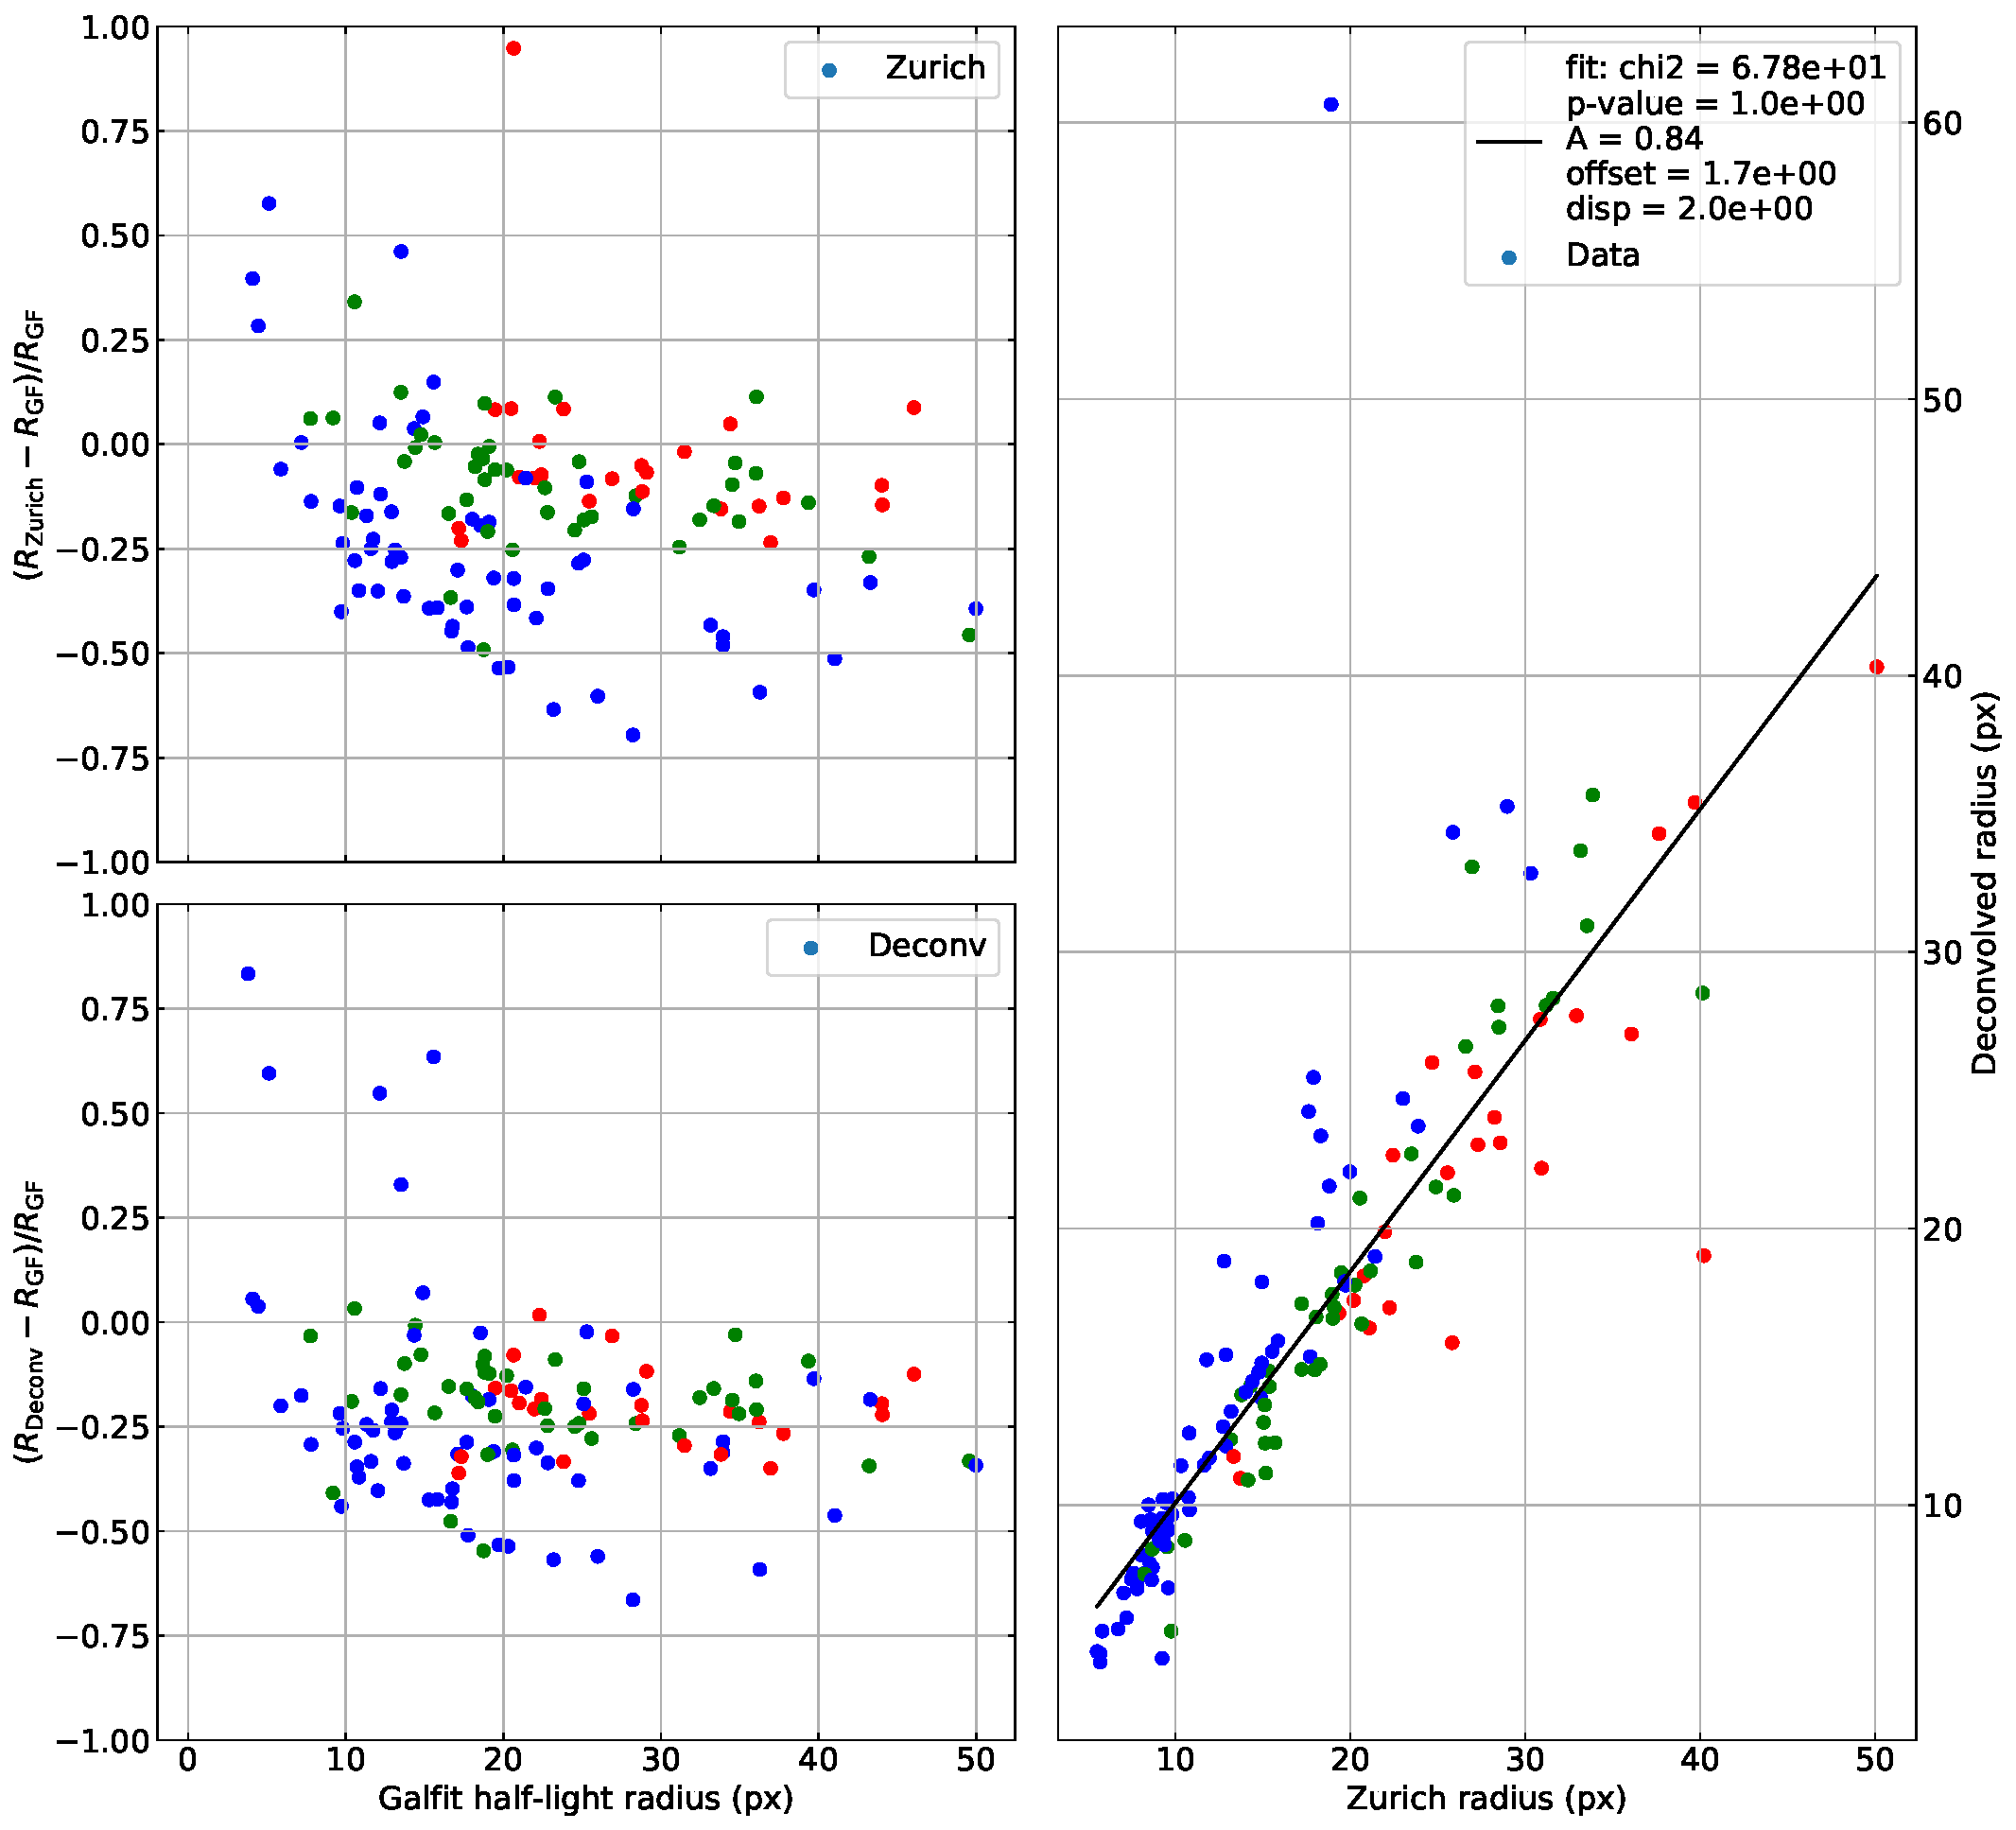
\includegraphics[width=0.66\linewidth]{plotsWithColourCoding/zurichAndDeconvolvedRadii_against_Galfit_colourCodedWithCassataType.pdf}	
	    \caption{Haut gauche : difference relative entre le rayon effectif de Zurich et celui de GalFit en fonction du rayon de GalFit. Bas gauche : même graphe avec le rayon déconvolué. Droite : rayon déconvolué en fonction de celui de Zurich.}
	     \label{fig:comp_Zurich_deconvolue}
    \end{figure}    
    
    
   
    

\end{document}